\section{Radio Simulation}\label{sec:radiomodel}
\bibtodo{slight changes from original}
To simulate loss of packets during radio communication, we introduce the packet error probability. The packet
error probability is the probability for any form of error occurring during the transmission and reception of
a packet through wireless radio communication. The probability for packet error is calculated using the
\gls{rssi} on a link between two nodes, the size of the packet, as well as the \gls{snr}, including
interference from nearby transmitting nodes. The computations in this section are derived from
\cite{massoud2007digital}, as well as personal communication with the author of \cite{paper:linkmodel}.

\subsection{Probability for Packet Error}\label{sec:pep}
The first step for computing the probability for packet error is to compute the level of background noise
affecting the wireless communication, the noise power $P_{N,\mathit{dB}}$. This noise is calculated with the
thermal noise and noise figure $P_{N,\mathit{dB}} = \mathit{thermalnoise}\ +\ \mathit{noisefigure}$. For the
Reachi devices we assume that the $\mathit{thermalnoise} = -119.66$ \acrshort{db} and the
$\mathit{noisefigure} = 4.2$ \acrshort{db}. Next, we need to add the noise from interfering transmissions
happening at the same time. This is done by adding the sum of the \gls{rssi} from interfering transmitters to
the noise power $P_{N,\mathit{dB}}$, giving us the noise power with interference $P_{NI,\mathit{dB}}$ on the
specific link between a receiving node $n_r$ and a transmitting node $n_t$ at a given time $t$. The set of
currently transmitting and interfering nodes are denoted by $\mathit{nodes}_i$ and the the function
$\mathit{RSSI}_{\mathit{dBm}}(n, m, t)$ denotes the \gls{rssi}, in \acrshort{dbm}, on the link between nodes
$n$ and $m$ at time $t$. We assume the \gls{rssi} on a link to be reciprocated, which means that
$\mathit{RSSI}_{\mathit{dBm}}(n, m, t) = \mathit{RSSI}_{\mathit{dBm}}(m, n, t)$.

\begin{eq}\label{eq:noisepower}
    P_{NI,\mathit{dB}}(n_r, m_t, \mathit{nodes}_i, t) = 10 \log_{10}\left( 10^{\frac{P_{N,\mathit{dB}}}{10}} +
    \mathlarger{\sum}\limits_{m \in \mathit{nodes}_i}  10^{\frac{\mathit{RSSI}_{\mathit{dBm}}(n_r, m, t)}{10}}
    \right)
\end{eq}

Note that as both the noise power $P_{N,\mathit{dB}}$ and the \gls{rssi} is in \acrshort{db} (a logarithmic
scale), we first need to convert the values to a linear scale, before we can compute the sum of the background
noise and the interfering noise, and then finally convert the value back into a logarithmic scale. \medbreak

With the noise and interference power $P_{NI,\mathit{dB}}$, we can compute the \gls{snir},
$\gamma_{\mathit{dB}}$. The \gls{snir} compares the \gls{rssi} of the signal to the level of the background
noise, as well as the noise from interfering transmitters. The ratio is computed by subtracting the noise
power $P_{NI,\mathit{dB}}$ from the \gls{rssi} of a link.

\begin{eq}
    \gamma_{\mathit{dB}}(n_r, m_t, \mathit{nodes}_i, t) = \mathit{RSSI}_{\mathit{dBm}}(n_r, m_t, t) -
    P_{NI,\mathit{dB}}(n_r, m_t, \mathit{nodes}_i, t)
\end{eq}

We use the \gls{snir} $\gamma_{\mathit{dB}}$ to compute the bit error probability $P_b$:

\begin{eq}
    P_b(n_r, m_t, \mathit{nodes}_i, t) = \frac{1}{2}\mathit{erfc} \left( \sqrt{ \left(
    \frac{10^{\frac{\gamma_{\mathit{dB}}(n_r, m_t, \mathit{nodes}_i, t)}{10}}}{2} \right)} \right)
\end{eq}

Finally, with the bit error probability $P_b$, we can compute the packet error probability $P_p$. The packet
error probability is the probability that we experience a bit error for any of the bits in the transmitted
packet.

\begin{eq}\label{eq:pep}
    P_p(n_r, m_t, \mathit{nodes}_i, \mathit{packetsize}, t) = 1 - \left( 1 - P_b(n_r, m_t, \mathit{nodes}_i,
    t) \right) ^{\mathit{packetsize} \cdot 8}
\end{eq}

\subsection{Example}
If we assume that a node $n_2$ is currently listening, and nodes $n_1$ and $n_3$ is transmitting at the same
time $t$, what is the probability for a packet error on the link between nodes $n_1$ and $n_2$ with
interference $\mathit{nodes}_i = \{ n_3 \} $? For this example we assume the \gls{rssi} for the link between
$n_1$ and $n_2$ to be $\mathit{RSSI}_{\mathit{dBm}}(n_2, n_1, t) = -63.750$, the \gls{rssi} between $n_2$ and
$n_3$ to be $\mathit{RSSI}_{\mathit{dBm}}(n_2, n_3, t) = -74.042$, and the size of the transmitted packet to
be 20 bytes (which is the size of a header packet for the Reachi protocol). First, we compute the noise power 
$P_{\mathit{NI}, \mathit{dB}}$:
\begin{eq}
    P_{\mathit{NI},\mathit{db}}(n_2, n_1, \mathit{nodes}_i, t) = 10 \log_{10}\left( 10^{\frac{(-119.66 + 4.2)}{10}} + 10^{\frac{-74.042}{10}} \right) = -74.041
\end{eq}

We subtract the noise power $P_{NI,dB}$ from the \gls{rssi} to get the \gls{snir} $\gamma_{dB}$:
\begin{eq}
    \gamma_{\mathit{dB}}(n_2, n_1, \mathit{nodes}_i, t) = -63.750 - (-74.041) = 10.291
\end{eq}

With which we can compute the bit error probability:
\begin{eq}
    P_b(n_2, n_1, \mathit{nodes}_i, t) = \frac{1}{2}erfc \left( \sqrt{ \left( \frac{10^{\frac{10.291}{10}}}{2} \right)} \right) = 0.000537
\end{eq}

Finally we can compute the packet error probability using the bit error probability:
\begin{eq}
    P_p(n_2, n_1, \mathit{nodes}_i, t, 20) = 1 - \left( 1 - 0.000537 \right) ^{20 \cdot 8} = 0.082
\end{eq}

This gives us an 8.2 \% probability that we will experience a packet error during the transmission from $n_1$
to $n_2$ with interference from $n_3$, which is a significant difference in relation to the same transmission
with no interfering transmitters. To demonstrate the difference, \autoref{plot:radiomodel:no-interference}
shows the probability for packet error with no interfering transmitters. According to the figure, an
\gls{rssi} of approximately $-103.0$ \acrshort{dbm} would have a probability for packet error close to zero,
and an \gls{rssi} of approximately $-110.0$ \acrshort{dbm} would have a probability for packet error very
close to 100.0 \%. Recall that for the link between $n_1$ and $n_2$ at time $t$, we had an \gls{rssi} of
$-63.750$ \acrshort{dbm}, which is significantly better than the $-103.0$ \acrshort{dbm} we see in
\autoref{plot:radiomodel:no-interference} for a close to zero probability, but with just a single interfering
transmitter, the probability for packet error increases to 8.2 \%, which corresponds to what we see in
\autoref{plot:radiomodel:one-interference}, where and \gls{rssi} of approximately $-62.0$ \acrshort{dbm} is 
required for a probability for packet error close to zero, with a single interfering transmitter.

\begin{figure}[H]
    \centering
    \begin{subfigure}[t]{.9\textwidth}
        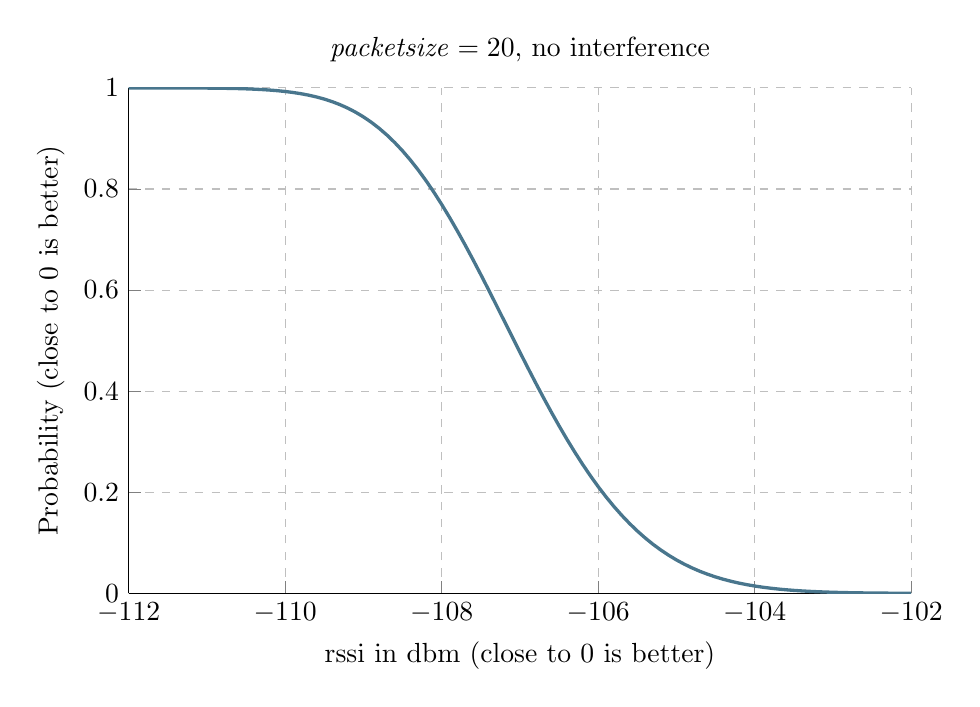
\begin{tikzpicture}%\label{plot:reachi-experiments:average-distance}
            \begin{axis}[
                    title={$\mathit{packetsize} = 20$, no interference},
                    height=8cm, width=0.95\textwidth,
                    ylabel={Probability (close to 0 is better)},
                    xlabel={\gls{rssi} in \acrshort{dbm} (close to 0 is better)},
                    axis lines*=left,
                    enlargelimits=false,
                    xtick={-112, -110, -108, -106, -104, -102},
                    ymajorgrids=true,
                    xmajorgrids=true,
                    grid style=dashed,
                ]
    
                \addplot[very thick, solid, cyan!50!black] coordinates {(-112,0.9999876428126551)(-111.9,0.9999818533805854)(-111.8,0.9999735236168629)(-111.7,0.9999616235974554)(-111.6,0.9999447451717537)(-111.5,0.999920980149257)(-111.4,0.9998877661533198)(-111.3,0.999841694145744)(-111.2,0.9997782714374498)(-111.1,0.9996916341768787)(-111.0,0.9995742039839494)(-110.9,0.999416284715221)(-110.8,0.9992055974422288)(-110.7,0.9989267547148308)(-110.6,0.9985606791379564)(-110.5,0.9980839762217061)(-110.4,0.9974682772917275)(-110.3,0.9966795747809701)(-110.2,0.995677579153797)(-110.1,0.9944151335993024)(-110.0,0.9928377289131765)(-109.9,0.9908831660120753)(-109.8,0.9884814165838162)(-109.7,0.9855547327690343)(-109.6,0.9820180538712832)(-109.5,0.977779751436127)(-109.4,0.9727427433945262)(-109.3,0.966805993404494)(-109.2,0.9598663934709013)(-109.1,0.9518210071670542)(-109.0,0.9425696284608098)(-108.9,0.9320175886859855)(-108.8,0.9200787232079811)(-108.7,0.9066783914790133)(-108.6,0.8917564310398185)(-108.5,0.8752699189322612)(-108.4,0.8571956138868371)(-108.3,0.8375319599914338)(-108.2,0.8163005472222238)(-108.1,0.7935469455391158)(-108.0,0.769340856001552)(-107.9,0.7437755528934127)(-107.8,0.7169666232111204)(-107.7,0.6890500419860338)(-107.6,0.6601796517461043)(-107.5,0.6305241401480931)(-107.4,0.6002636299578492)(-107.3,0.5695860091061149)(-107.2,0.5386831349945436)(-107.1,0.5077470465831848)(-107.0,0.4769663105493268)(-106.9,0.4465226148609678)(-106.8,0.4165877056515772)(-106.7,0.3873207426887495)(-106.6,0.35886612643390514)(-106.5,0.3313518270787408)(-106.4,0.3048882242599883)(-106.3,0.27956744643051556)(-106.2,0.25546318188223016)(-106.1,0.23263091968407745)(-106.0,0.21110856856704174)(-105.9,0.19091739506360728)(-105.8,0.17206321880579134)(-105.7,0.15453780245757087)(-105.6,0.13832037585666812)(-105.5,0.12337923806141704)(-105.4,0.10967338661475745)(-105.3,0.09715412994657713)(-105.2,0.08576664597225181)(-105.1,0.07545145721250357)(-105.0,0.06614579982676905)(-104.9,0.057784870567569646)(-104.8,0.050302941646255594)(-104.7,0.04363433873657152)(-104.6,0.037714281778700065)(-104.5,0.032479591872253466)(-104.4,0.027869270393728107)(-104.3,0.023824958598936963)(-104.2,0.0202912874470752)(-104.1,0.017216128297656508)(-104.0,0.014550755569625706)(-103.9,0.012249932504283412)(-103.8,0.010271930917551964)(-103.7,0.00857849534048738)(-103.6,0.007134761292770797)(-103.5,0.005909136667815562)(-103.4,0.004873154377310507)(-103.3,0.004001303543972212)(-103.2,0.003270845672304956)(-103.1,0.002661621391885305)(-103.0,0.00215585257009554)(-102.9,0.0017379438436174732)(-102.8,0.0013942869261214241)(-102.7,0.0011130704181615547)(-102.6,0.0008840972739669883)(-102.5,0.000698611570752572)(-102.4,0.0005491357749322079)(-102.3,0.0004293193051855271)(-102.2,0.00033379885272988297)(-102.1,0.0002580706275865374)(-102.0,0.0001983744574920454)};
    
            \end{axis}
        \end{tikzpicture}
       \caption{Probability for packet error on a link with no interfering transmitters.}\label{plot:radiomodel:no-interference}
    \end{subfigure}
    \begin{subfigure}[t]{.9\textwidth}
        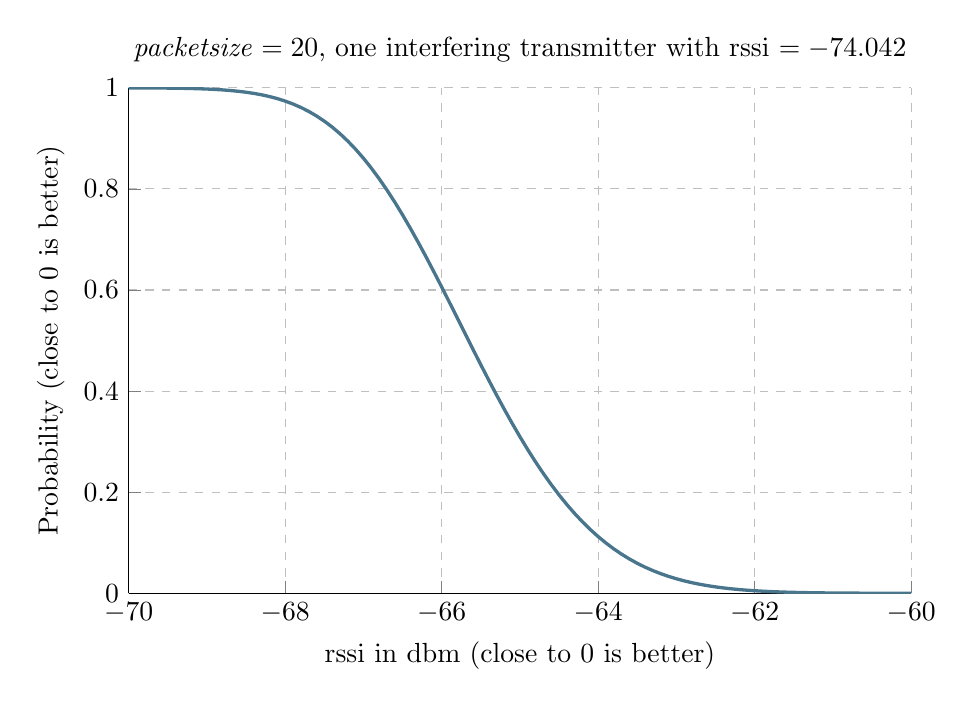
\begin{tikzpicture}%\label{plot:reachi-experiments:average-distance}
            \begin{axis}[
                 title={$\mathit{packetsize} = 20$, one interfering transmitter with \gls{rssi} $= -74.042$},
                    height=8cm, width=0.95\textwidth,
                    ylabel={Probability (close to 0 is better)},
                    xlabel={\gls{rssi} in \acrshort{dbm} (close to 0 is better)},
                    axis lines*=left,
                    enlargelimits=false,
                    xtick={-70, -68, -66, -64, -62, -60},
                    ymajorgrids=true,
                    xmajorgrids=true,
                    grid style=dashed,
                ]
                
                \addplot[very thick, solid, cyan!50!black] coordinates
                {(-70,0.9998946969201213)(-69.9,0.999851280175236)(-69.8,0.9997914288482014)(-69.7,0.9997095541645235)(-69.6,0.9995984200856673)(-69.5,0.9994487512548663)(-69.4,0.999248779311367)(-69.3,0.9989837280265265)(-69.2,0.9986352414918488)(-69.1,0.9981807643451096)(-69.0,0.997592888694345)(-68.9,0.9968386888236752)(-68.8,0.9958790716514758)(-68.7,0.9946681778438871)(-68.6,0.9931528749262344)(-68.5,0.9912723890419786)(-68.4,0.9889581254816121)(-68.3,0.9861337290346813)(-68.2,0.9827154329627786)(-68.1,0.9786127394483093)(-68.0,0.973729464463402)(-67.9,0.9679651661382458)(-67.8,0.9612169582453458)(-67.7,0.9533816900793851)(-67.6,0.9443584518788336)(-67.5,0.9340513423828241)(-67.4,0.9223724137305926)(-67.3,0.9092446903599295)(-67.2,0.894605144450226)(-67.1,0.8784075021721859)(-67.0,0.8606247535759753)(-66.9,0.841251244920013)(-66.8,0.8203042456090053)(-66.7,0.7978249020903394)(-66.6,0.7738785169287781)(-66.5,0.74855412125948)(-66.4,0.7219633410028916)(-66.3,0.6942385895436469)(-66.2,0.6655306499723479)(-66.1,0.6360057365895722)(-66.0,0.6058421466303818)(-65.9,0.5752266279786769)(-65.8,0.5443505964027997)(-65.7,0.5134063364756047)(-65.6,0.48258331425256296)(-65.5,0.4520647177980315)(-65.4,0.422024324919833)(-65.3,0.392623777345657)(-65.2,0.36401031848479315)(-65.1,0.33631502926640344)(-65.0,0.3096515746076566)(-64.9,0.2841154529163329)(-64.8,0.25978372350145207)(-64.7,0.2367151724125871)(-64.6,0.2149508663479005)(-64.5,0.19451503691409577)(-64.4,0.17541623353097346)(-64.3,0.1576486823314981)(-64.2,0.14119379008160704)(-64.1,0.1260217359331075)(-64.0,0.11209309920507793)(-63.9,0.09936047785157087)(-63.8,0.08777005934655302)(-63.7,0.07726311298604938)(-63.6,0.06777737973327802)(-63.5,0.05924834244541988)(-63.4,0.05161036543000741)(-63.3,0.04479769765769026)(-63.2,0.038745338542438446)(-63.1,0.03338976897292556)(-63.0,0.02866955326566123)(-62.9,0.024525819961693007)(-62.8,0.02090263097826983)(-62.7,0.017747249636844042)(-62.6,0.015010318608602913)(-62.5,0.012645958934183965)(-62.4,0.010611801070009363)(-62.3,0.008868958463135512)(-62.2,0.007381953529277174)(-62.1,0.006118605158747625)(-62.0,0.00504988605383716)(-61.9,0.004149757343889449)(-61.8,0.0033949870645402225)(-61.7,0.0027649582456965582)(-61.6,0.002241471548095064)(-61.5,0.0018085466304298414)(-61.4,0.0014522257270703776)(-61.3,0.0011603822729023827)(-61.2,0.0009225368308002357)(-61.1,0.0007296820553771566)(-61.0,0.0005741179660628815)(-60.9,0.0004492983977033571)(-60.8,0.0003496891470554653)(-60.7,0.0002706380340258274)(-60.6,0.00020825684500058728)(-60.5,0.0001593149176219999)(-60.4,0.00012114395831475111)(-60.3,9.15535532985956e-05)(-60.2,6.875673521467007e-05)(-60.1,5.130489908311553e-05)(-60.0,3.803131895474543e-05)};
    
            \end{axis}
        \end{tikzpicture}
       \caption{Probability for packet error on a link with a single interfering transmitter.}\label{plot:radiomodel:one-interference}
    \end{subfigure}
    \caption{Probability for packet error with and without interfering transmitters.}
    \label{figure:pepegraphs}
\end{figure}
